%%%%%%%%%%%%%%%%%%%%%%%%%%%%%%%%%%%%%%%%%%%%%%%%%%%%%%%%%%%%%%%%%%% 
%                                                                 %
%                            CHAPTER FOUR   - Reasoning Agent - Version 2            %
%                                                                 %
%%%%%%%%%%%%%%%%%%%%%%%%%%%%%%%%%%%%%%%%%%%%%%%%%%%%%%%%%%%%%%%%%%% 
 
\chapter{Version 2 (Work to be Done) - A Reasoning Agent Using an Auto-Generated KB}

In this section, more detail of the methods used for programmatically generating the knowledge
base and the agent will be discussed, specifically, the techniques by which assertions will be 
extracted from the text corpus (CFE Manual) and the battery of multiple choice questions.  Note that
in this second version, the battery of 1500 mutiple choice questions that make up the study package 
for the CFE exam will be divided into a 1300 question ``training'' set and a 200 question test set.
The 1300 question training set will be used for relation extraction as well as for any machine learning
algorithms that may be deemed appropriate as the project moves forward.  So, the term, ``training'', 
here, is used rather loosely as a catch-all for all forms of mechanized information gathering about the
problem domain.

\section{Programmatic Knowledge Base Development}

The assertions within
this knowledge base will largely be similar in format to Resource Description Format (RDF) triples, identifying entities and relations between them.  There may, however, also be assertions regarding the 
probabilities associated with answer types associated with certain question types.  Further detail is 
provided below.

\subsection{Entity Identification}

Certainly, relation extraction and entity identification is a major open area of research, currently.  A 
number of techniques have been devised, including Hearst 1992 \cite{hearst1992automatic}, or that used in Prismatic 2010 \cite{fan2012automatic}, for rule-based relation extraction.  Other, known machine learning based techniques may be employed as well,
if proven effective.  In addition, however, the techniques that exploit the structure of the 
information resources will be used, as described below.

\subsubsection{CFE Manual}

The CFE Manual, the definitive study guide for the CFE exam, is a text corpus structured as a text book.
As such, it is structured hierarchically, as any text book is, complete with features embedded in the text
that make this hierarchy apparent.  The most obvious feature is the table of contents.  In fact, the CFE 
Manual has a number of tables of contents, including a main table of contents, at the front of the manual,
and a set of area-specific tables of contents - one for each of the major test areas - Financial Transactions
and Fraud Schemes, Law, Investigation, and Fraud Prevention and Deterrence.  The combination of these
tables of contents provides an excellent window into entities that exist in the problem domain and the 
relations between them.  

As an example, consider Figure~\ref{fig:cfe_manual_toc} which shows a section of the table of contents 
relating to subject of Financial Statement Analysis.  It is readily apparent from this that there are hierarchical relationships between, for example, Financial Statement Analysis and Ratio Analysis.  Further,
there is a nice breakdown of the types of Common Financial Ratios - Current Ratio, Quick Ratio, etc.  Each 
of these pairs of hierchical entries establish a relation - either a type-of or part-of relation the exact
nature of which may be construed from other features, including the titles of the sections, the text
associated with these sections, or even the capitalization of these sections.  (For example, it's commonly
the case throughout the manual that fully capitalized subsections, (such as, QUICK RATIO) are generally type-of entities of their parent sections.)

\begin{figure}
\centering
\vspace{2.0in}
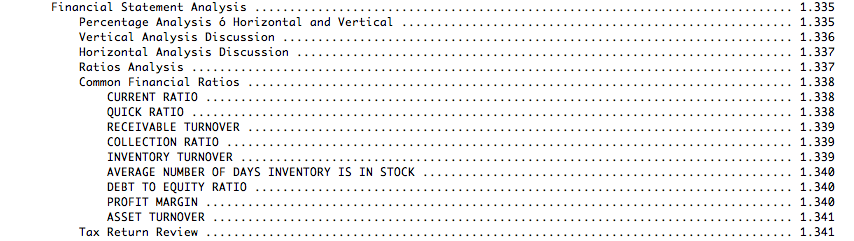
\includegraphics[width=150mm]{cfe_manual_toc.png}
\caption{A section of the table of contents from the CFE Manual}
\label{fig:cfe_manual_toc}
\end{figure}


\subsubsection{CFE Exam Questions}

\begin{figure}
\centering
\vspace{2.0in}
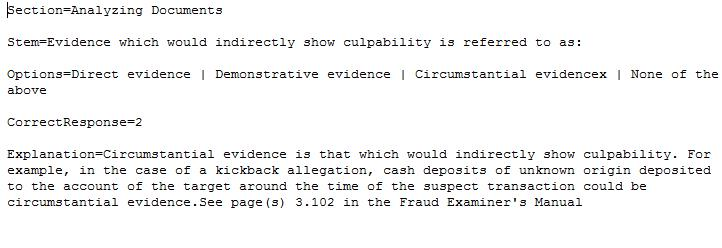
\includegraphics[scale=0.75]{study_package_formatted_text.jpg}
\caption{Scrubbed Practice Question}
\label{fig:study_package_formatted_text_2}
\end{figure}

Consider Figure~\ref{fig:study_package_formatted_text_2}, which shows the same formatted question as 
Figure~\ref{fig:study_package_formatted_text}, discussed above.   This question provides a typical 
example of the sorts of semantically relevant information that can be extracted from multiple choice
questions, in general.  First, notice that substituting the correct answer, option 2, ``Circumstantial 
evidence'', in for the term ``Evidence'' in the stem gives a S-V-O relation, i.e., 
shows(circumstantial-evidence, culpability).  Second, each of the options names various entities, all of 
which are types of evidence (except for the None of the Above option).  This is typically the case with multiple choice questions - the incorrect answers typically are relevant to the domain, and are often
the same entity type as the correct answer.  And in general, all of the options are siblings of each
other in the domain ontology.  This is also of value - if this information wasn't already made evident
in the structure of the manual, it is certainly made obvious here, and can then be used to cross-reference
with the manual to make further inferences.

Next, there's the issue of not-assertions.  That is, given that option 2 is the correct answer, it is 
implied that each of the other options are not the correct answer.

Finally, there's the information of the explanation, whose focus gives a definition of the correct option,
circumstantial evidence.  Here, too, is information that could be used as meta data, pertaining to the 
words associated with the definition of circumstantial - indirect, culpability.  


\subsection{Metadata}

Metadata can take many forms.  Among them is the information associated with information retrieval
techniques, as discussed below.  The metadata discussed here as well as any other such information
that are shown valuable may be used, and added to the knowledge base.

\subsubsection{Information Retrieval}

Among methods for programmatically collecting meta-data are information retrieval (IR) techniques, 
which glean various pieces of shallow language information, which regardless of their shallow depth provide possible data points on which the reasoning agent can make inferences.  The key idea is to break up the CFE Manual into a series of hierarchical documents, (based on its table of contents, and syntax features), as shown in Figure~\ref{fig:document_collection}.  Then, collect IR information from each document, including (but not limited to) term frequency, document frequency, language model, and document features \cite{manning2008introduction}.  Term frequency is simply the count of each term in the document, document frequency refers to the number of documents that a given term appears in.  Language model refers to the probabilistically based unigram, bigram, and trigrams in the document, which can be compared with those embedded in a question to be answered by the agent.  Document features refer to various features such as the document's location in the document hierarchy, whether its title is all caps, etc.

\begin{figure}
\centering
\vspace{2.0in}
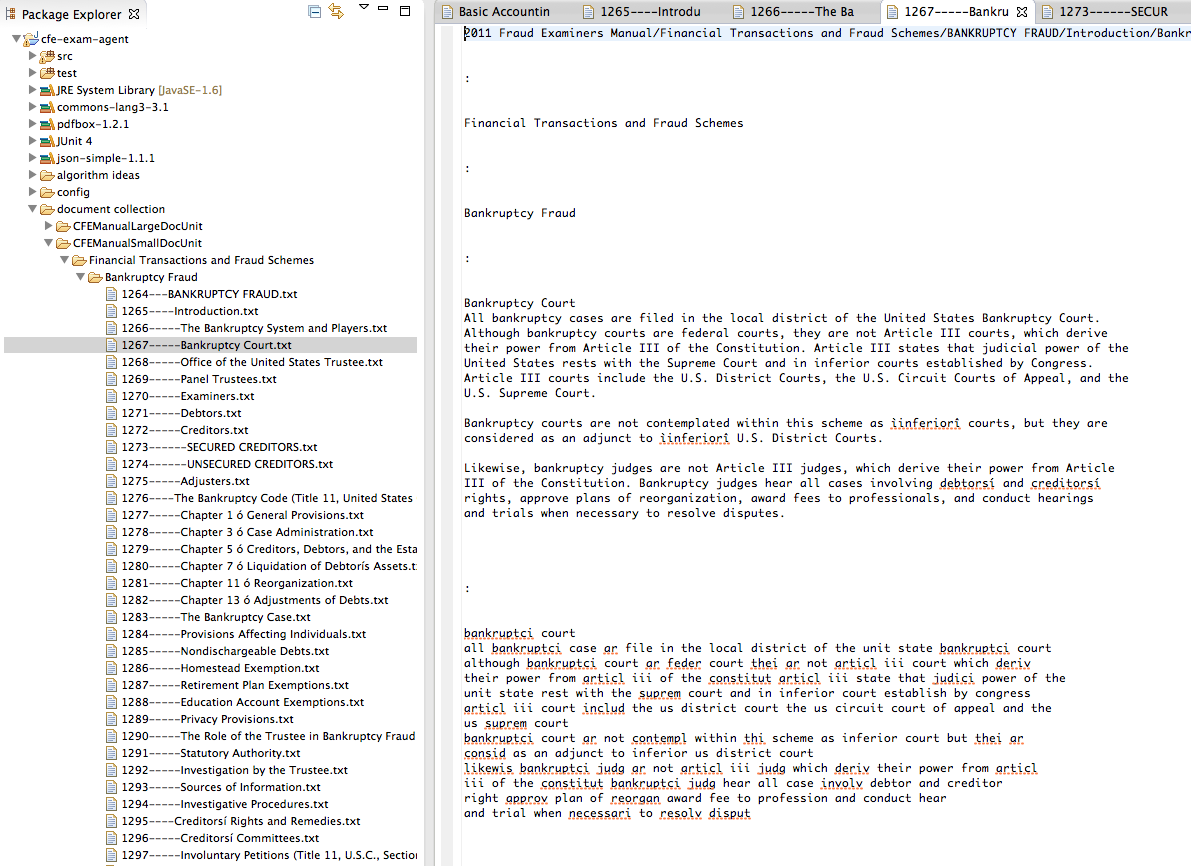
\includegraphics[width=150mm]{document_collection.png}
\caption{The CFE Manual as a Document Collection}
\label{fig:document_collection}
\end{figure}

\section{Reasoning with Uncertainty}

The reasoning agent will be dealing with uncertainty as it makes decisions during the exam.  Further,
there will likely be degrees of uncertainty to be made explicit as relations are discovered (which measure
the degree of certainty of the validity of the relations).  As such, various tools for handling uncertainty
in a formal way include, but are not limited to the following.

\begin{itemize}
\item Probabilistic Logic \cite{nilsson1986probabilistic}

\item Markov Logic \cite{richardson2006markov}

\item Dempster Schaffer \cite{yager1987dempster}

\end{itemize}

The best way to handle this will be addressed as the project moves forward.


\section{Verification}

There is a history of efforts to create agents that perform well on tests in the spirit of an interpretation of artificial intelligence called ``Psychometric AI''\cite{psychoai.ijcai03, bringsjord_jetai_pai_overview_2011, Bringsjord2012}.  Psychometric AI (PAI) is grounded in the notion that by making machines that can pass tests, the machine can, in some sense, be called ``intelligent''\cite{psychoai.ijcai03}.  Although it's readily conceded that the ability to pass a particular test (or particular set of tests) is an inadequate basis for defining the full range of what it means to be intelligent, it does offer the very attractive element of concreteness\cite{psychoai.ijcai03, bringsjord_jetai_pai_overview_2011} --- a very appealing feature given the struggle one commonly has when attempting to delineate what it means to make machines that can ``think''.  After all, tests offer a number of concrete aspects --- a well-defined start, end, set of goals implied by the questions themselves, and ultimately, a score.  Psychometric AI, then, is the methodological basis for verification of the KB by measuring the performance of an agent
that uses the KB to answer test questions.

Among the 50+ testing sections on the exam, the question battery of 1500 questions will be broken
into two groups - the 1300 questions on which the training will be executed and the 200 questions
on which the reasoning agent will be tested.  This breakdown will be proportionate for each testing
section, assuring that all sections are represented in both the training set and in the test set.  That is,
every test area will have at least one question in both the training set and in the test set.


















